\begin{question}
  \hspace*{\fill} [Note Maximale: ?]\par
  \noindent Dans un parc d'attractions, une grande roue dont le diamètre est de 111 mètres tourne à une vitesse constante. Le bas de la roue est k mètres au-dessus du sol. Un siège part du bas de la roue.\par
  \medskip
  \begin{center} % or flushleft or flushright
    \noindent La figure n'est pas à l'échelle.\par
    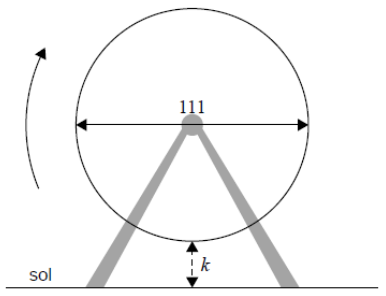
\includegraphics[scale=0.4]{figure_x20}\par
    \noindent La roue complète un tour en 16 minutes.\par
  \end{center} % or flushleft or flushright

  \noindent Après t minutes, la hauteur du siège au-dessus du sol est donnée par $h(t) = 61,5 + a\,Cos\left(\frac{\pi}{2}t\right)$, pour $0 \le t \le 32$.\par
  \begin{enumerate}[label=(\alph*)]
    \item Après 8 minutes, le siège est 117 m au-dessus du sol. Trouvez $k$\hspace*{\fill} [?]
    \item Trouvez la valeur de $a$.\hspace*{\fill} [?]
    \item Trouvez quand le siège est 30 m au-dessus du sol pour la troisième fois.\hspace*{\fill} [?]
  \end{enumerate}
\end{question}
